\section{MAPS}

    %%%%%%%%%%%%%%%%%%%%%%%%%%%%%%%%%%%%%%%%
    %%  Slide 1: <MAPS concept>  %%
    %%%%%%%%%%%%%%%%%%%%%%%%%%%%%%%%%%%%%%%%
    \begin{frame}
        \frametitle{Pixel detectors}
        \begin{itemize}
            \item caratteristiche standard e vantaggi rispetto agli ibridi?
        \end{itemize}
        3 strade diverse: MAPS, hybrid e CCDs.
    \end{frame} 

        %\tikz[remember picture] \node[coordinate,yshift=0.5em] (n1) {};  
        %\tikz[remember picture] \node[coordinate] (n2) {};




    %%%%%%%%%%%%%%%%%%%%%%%%%%%%%%%%%%%%%%%%
    %%  Slide 1: <CMOS MAPS concept>  %%
    %%%%%%%%%%%%%%%%%%%%%%%%%%%%%%%%%%%%%%%%
    \begin{frame}
        \frametitle{CMOS MAPS}
        \begin{multicols}{2}
            \begin{figure}[h!]
                \centering
                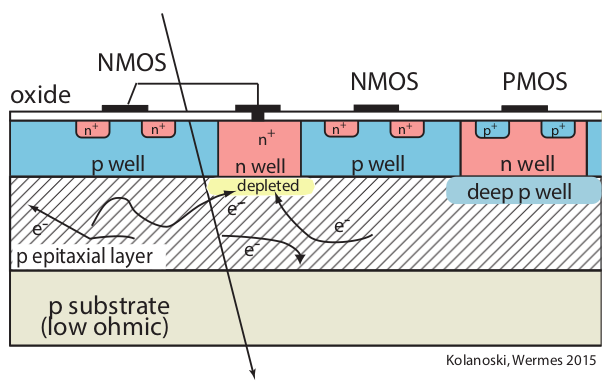
\includegraphics[width=.8\linewidth]{figures/Pixel_detectors/MAPS_scheme.png}
            \end{figure}
            \columnbreak
            \begin{tikzpicture}[overlay]
                %\path (n2) -| node[coordinate] (n3) {} (n1);
                \draw[decorate,decoration={brace,amplitude=8pt,raise=19pt}]
                      (0,0) -- (0,1);
            \end{tikzpicture}
            $\lesssim$\SI{5}{\um}\\
            $\lesssim$\SI{50}{\um}
            \begin{equation}
                d \propto \sqrt{\rho V}
            \end{equation}
        \end{multicols} 

        \begin{itemize}
            \item electronics is low resistivity while sensor needs high resistivity, special technologies for the sensor. Next slide!
            \item If not completed depleted charge is collected by diffusion
            \item very low Capacity
        \end{itemize}
        \end{frame} 

    %%%%%%%%%%%%%%%%%%%%%%%%%%%%%%%%%%%%%%%%
    %%  Slide 1: <>  %%
    %%%%%%%%%%%%%%%%%%%%%%%%%%%%%%%%%%%%%%%%
    \begin{frame}
        \frametitle{Sensor}
        \begin{figure}[h!]
            \centering
            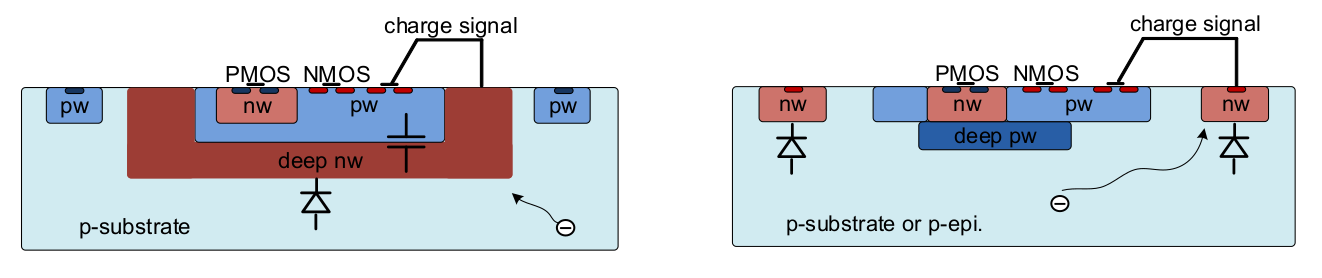
\includegraphics[width=.8\linewidth]{figures/Pixel_detectors/large_small_sensor_scheme.png}\\
            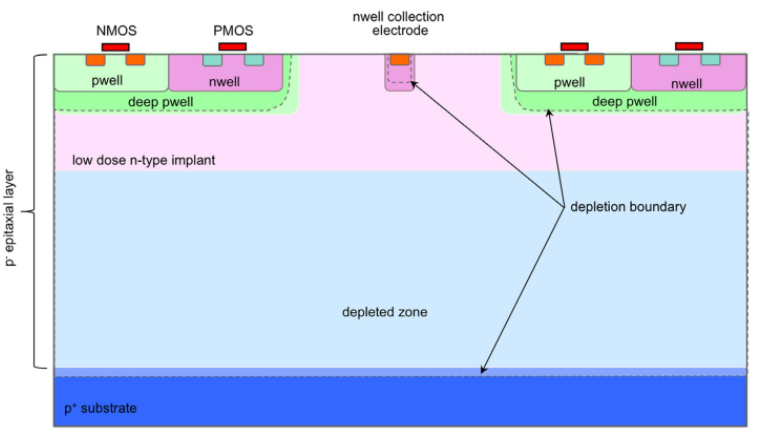
\includegraphics[width=.8\linewidth]{figures/Pixel_detectors/ALPIDE_after_PM.png}
        \end{figure}
        Pro e contro in termini di capacità e rumore. 
        High resistivity depleted epi layer, and process modification. 
    \end{frame} 

    %%%%%%%%%%%%%%%%%%%%%%%%%%%%%%%%%%%%%%%%
    %%  Slide 1: <>  %%
    %%%%%%%%%%%%%%%%%%%%%%%%%%%%%%%%%%%%%%%%
    \begin{frame}
        \frametitle{Readout}
        Front end on pixel. Very important task: dimension of components. 
        Microelectronics is alla base dello sviluppo dei MAPS. 
        
        Economia della pixel area. Many to take into account:
        \begin{itemize}
            \item sparsified readout allows for an optimization in the data trasnfer
            \item no rolling shut, but data push
            \item Column drain is one of the most popular readout mechanism, but other possible are possible
            \item memory on pixel!
        \end{itemize}
 
    \end{frame} 